\chapter{Evaluation}
The experiments were executed in three environments to keep the topology constant while varying the platform: an AWS cloud instance, a single physical Ubuntu host, and two physical Ubuntu hosts connected by an Ethernet link. Across all environments, the setup isolated components using Linux network namespaces and instantiated the three translators under test (Jool, Tayga, Tundra) with identical addressing and routing. Configuration choices such as forwarding and addressing were held consistent across environments to support comparability. 

\section{Test environments}
\paragraph{AWS}
In the AWS environment, a single EC2 instance within a dual-stack VPC hosted the entire virtual topology. Client, translator, and server roles were realized as separate namespaces interconnected by veth pairs\cite{veth4}. DNS64 and CLAT ran locally on the instance to avoid external dependencies, and the dual-stack baseline followed a direct namespace path that bypassed translation.

\paragraph{Bare-metal host}
On the bare-metal host, the same namespace-based topology was reproduced on bare metal. Client and server namespaces were connected via veth, translators were deployed in dedicated namespaces with uniform routing, and CLAT was instantiated to mirror the cloud setup. 
\paragraph{Bare-metal network}
In the bare-metal network setup, two Ubuntu machines were connected via a dedicated Ethernet link. The client machine hosted the namespace topology and the translator variants. The second machine provided a standard IPv4/IPv6 stack reachable over the Ethernet link. CLAT ran on the client machine, the dual-stack baseline traversed the link natively without translation. Hardware details and all configuration artifacts for these environments are provided in the Appendix.

\section{Networking Namespace Configuration}
The experiments relied on Linux networking namespaces to isolate each translator and to keep the surrounding network conditions reproducible across local and the cloud setup. For Tayga and Tundra, a single namespace per translator was connected to the host through a veth pair\cite{veth4}. Both ends of the veth received link-local IPv6 addresses and the namespace end additionally received a globally scoped IPv6 address. Inside the namespace, the default IPv6 route pointed to the host-side link-local address, while the host installed a route towards the namespace prefix via the namespace-side link-local address. IPv6 forwarding was enabled on the host and inside the namespaces to allow transit of translated traffic. 
Jool required a slightly different arrangement with two namespaces to create a single hop through the translator: an application namespace was linked to the translator namespace using a second veth pair. This common namespace wiring, addressing, and forwarding configuration was applied consistently on all machines so that the translator initialization in the next section could proceed without repeating network setup details.

\section{Implementation of Translation Technologies}
\paragraph{Tayga}
was implemented using a TUN device (nat64) inside a dedicated network namespace. Following Tayga’s stateless design, the translator was configured with the well‑known NAT64 prefix 64:ff9b::/96, one local IPv4 address for the CLAT side and one local IPv6 address for the NAT64 side, and a static one‑to‑one map to keep address selection deterministic. After creating and bringing up the nat64 device, the CLAT’s IPv4 was assigned as a /32 and an explicit route for the mapped IPv6 was installed. The namespace’s default IPv4 route was directed to the nat64 device so that IPv4‑only applications would traverse the translator, and IPv6 forwarding was enabled to forward translated packets toward the host‑side IPv6 path. This minimal setup produced a stable and reproducible CLAT path and integrated with the shared namespace wiring described previously. The configuration mirrors Tayga’s intended use as a simple, stateless NAT64 that offloads policy and state handling to the host’s packet filtering/NAT framework and is typically paired with DNS64 in practical deployments, which aligns with prior descriptions of Tayga’s design \cite{Repas_Farnadi_Lencse_2014,palrd_tayga_readme}.

\paragraph{Tundra} 
was deployed as a user‑space, stateless CLAT translator built from source with CMake and gcc and operated via the Linux TUN driver, consistent with its SIIT design and multi-threaded architecture \cite{rfc7915,labuda_tundra_nat64}. Address synthesis used the well-known 64:ff9b::/96 prefix, and translation of private IPv4 addresses was enabled to prevent corner cases during testing. The TUN interface was named “clat”, configured with static local endpoints. The interface was brought up, an explicit route to the CLAT IPv6 address was added, and the namespace’s default IPv4 route was set over the TUN interface. IPv6 forwarding was enabled to allow translated traffic to leave to the host’s IPv6 domain. This configuration yielded a minimal user-space CLAT setup comparable in spirit to Tayga\cite{labuda_tundra_nat64}.

\paragraph{Jool}
was deployed as a kernel-space, stateless SIIT translator in its own network namespace and paired with a separate application namespace to enforce a single hop through the translator. The namespaces were connected by a veth pair configured as an IPv4 link with additional IPv6 addresses on the same link, while a second veth pair connected the Jool namespace to the host and carried an IPv6 address. 

\begin{figure}[H]
    \centering
    \caption{Jool network namespace architecture with dual veth pairs.}
    \label{fig:jool_architecture}
    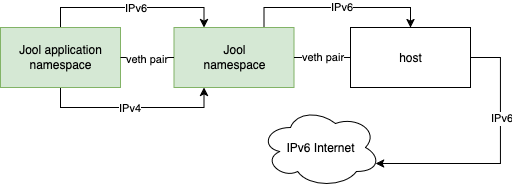
\includegraphics[width=0.8\textwidth]{resources/images/updatedjooldiagram.png}
\end{figure}

IPv4 and IPv6 forwarding were enabled in both host and Jool namespaces, the application namespace used a default IPv4 gateway so that all IPv4 flows traversed the translator, and IPv6 followed the link-local default routing pattern established earlier. Inside jool-ns (networking namespaces where jool was configured, not the namespace for the application), the jool\_siit module was loaded and a SIIT instance was created in Netfilter mode with pool6 set to \texttt{64:ff9b::/96}. An explicit Address Mapping Table entry bound the application’s IPv4 address to the Jool-side IPv6 address to keep the translation deterministic for the measurements. This choice of Netfilter mode, where inbound packets are greedily intercepted within the namespace, kept the configuration minimal while ensuring a low-overhead kernel datapath comparable to the user-space translators\cite{jool_introduction}. Given Jool’s SIIT/CLAT capabilities the setup aligns with the stateless translation model defined by SIIT \cite{jool_introduction,rfc7915}.


\section{Measurement Methodology}
\paragraph{Throughput} was measured with iperf3 (version 3.16) using a dedicated namespace (iperf-ns). The namespace was connected to the host via a veth pair, both ends received IPv6 link-local addresses, and the namespace end was assigned an IPv6 address. The namespace installed a default IPv6 route toward the host’s link-local address, while the host added routes to the translator prefixes over the same link. To enable NAT64-based reachability for an IPv4-only target within a stateless translation model, the well-known NAT64 prefix 64:ff9b::/96 was used to embed 192.0.0.171 as 64:ff9b::192.0.0.171, which was configured on iperf-ns so the server could accept both native IPv6 and synthesized IPv6 connections\cite{rfc7915}. An iperf3 server ran inside iperf-ns, and clients were executed from tayga-ns, tundra-ns, and jool-app-ns as defined in Sections 4.2–4.3.

The measurement plan separated a native IPv6 baseline from the CLAT translation paths. The IPv6 target provided a no-translation baseline whose purpose was to show pure topology effects, in particular the extra namespace hop in the Jool setup compared to the single-hop topologies of Tayga and Tundra. In contrast, the IPv4 target is the focus of this evaluation: client traffic started as IPv4 inside each namespace and was translated by the respective CLAT implementation, enabling a direct comparison of Tayga, Tundra, and Jool and, secondarily, a comparison to the IPv6 baseline to measure how much of any difference came from translation versus hop count. All tests used iperf3 over TCP with two durations (30 s and 120 s) to capture short and sustained behavior. The same scripts and parameters were applied on all three environments. 

\paragraph{RTT} was measured with ICMP echo using a simple harness that iterates over namespaces and targets, executes ping inside each namespace, and stores raw outputs for later plotting. Two targets were probed: the IPv4 address (the CLAT case of interest) and the IPv6 address (baseline). The IPv6 baseline is included for completeness consistent with the TCP tests.
For each run, the script selects ping (version iputils 20240117) or ping -6, uses a 1 s send interval and a deadline of 30s. The IPv4 measurements originate as IPv4 inside the namespace and are translated by the local CLAT toward the host-side IPv6 path. Replies are translated back by the same CLAT. The IPv6 target is reached natively without translation. 
